% Auriga theme
% https://github.com/anishathalye/auriga

\documentclass[14pt,aspectratio=169]{beamer}
\usepackage{pgfpages}
\usepackage{fancyvrb}
\usepackage{booktabs,dcolumn}
\usepackage{tikz}
\usetikzlibrary{arrows.meta, positioning, quotes}
\usepackage{pgfplots}

% \ifnotes
% \setbeamertemplate{note page}[plain]
% \setbeameroption{show notes on second screen=right}
% \fi

\usetheme{auriga}
\usecolortheme{auriga}

% define some colors for a consistent theme across slides
\definecolor{red}{RGB}{181, 23, 0}
\definecolor{blue}{RGB}{0, 118, 186}
\definecolor{gray}{RGB}{146, 146, 146}

\title{Historia Económica Argentina}

\author{\underline{Sebastián Freille} \inst{1}}

\institute[shortinst]{\inst{1} IEF-UNC \\ UCC}
\date{}

\AtBeginSection[]{
    \begin{frame}
    \vfill
    \centering
    \begin{beamercolorbox}[sep=8pt,center,shadow=true,rounded=true]{title}
        \usebeamerfont{title}\insertsectionhead\par%
    \end{beamercolorbox}
    \vfill
    \end{frame}
}



\AtBeginSubsection[]{
    \begin{frame}
    \vfill
    \centering
    \begin{beamercolorbox}[sep=6pt,center,shadow=true,rounded=true]{title}
        \usebeamerfont{title}\insertsubsectionhead\par%
    \end{beamercolorbox}
    \vfill
    \end{frame}
}


\AtBeginSubsubsection[]{
    \begin{frame}
    \vfill
    \centering
    \begin{beamercolorbox}[sep=4pt,center,shadow=true,rounded=true]{title}
        \usebeamerfont{title}\insertsubsubsectionhead\par%
    \end{beamercolorbox}
    \vfill
    \end{frame}
}


\begin{document}

{
  % rather than use the frame options [noframenumbering,plain], we make the
  % color match, so that the indicated page numbers match PDF page numbers
  \setbeamercolor{page number in head/foot}{fg=background canvas.bg}
  \begin{frame}
    \titlepage
  \end{frame}
}

  
  \section{Capítulo 2. La Gran Depresión y el impacto en Argentina:
    Aspectos macroeconómicos: fiscales y monetarios}


  \subsection{La evolución del sistema monetario y bancario desde 1880}


 \begin{frame}\frametitle{Convertibilidad interna y externa}
    \begin{itemize}\itemsep 10pt
      \item Entre 1914 y 1927 la moneda argentina fue inconvertible
        $\longrightarrow$ reservas de oro no corrían riesgo --ni
        drenaje externo (papel por oro) ni interno (depósitos por oro)
        \item ¿Al considerar la posible vuelta al patrón oro, se tenía
          noción de una posible corrida contra el sistema bancario y
          contra la CdC?
          \item ¿Qué tipo de régimen monetario y bancario es el
            óptimo para un economía pequeña y abierta?
                 \end{itemize}
      \end{frame}
  
      

 \begin{frame}\frametitle{Los dilemas de una economía pequeña y abierta}
   \begin{block}{Economía pequeña y abierta con TCFi}
     la adopción de TCFi suele ser motivada por un deseo de suavizar
     fluctuaciones extremas de precios externos y/o disciplinar las
     políticas locales en contextos inflacionarios. Cualquiera sea la
     forma del régimen de TCFi, el dilema central del nexo
     dinero-bancos está siempre latente: cómo pueden lograrse
     \textit{simultáneamente} la convertibilidad externa --TCFi- y la
     convertibilidad interna --sistema bancario de reservas
     fraccionarias. 
     \end{block}
      \end{frame}
  
      

  \begin{frame}\frametitle{El perfil del BNA}
\begin{figure}[hxtbp]\vspace{0cm}
  \centering
  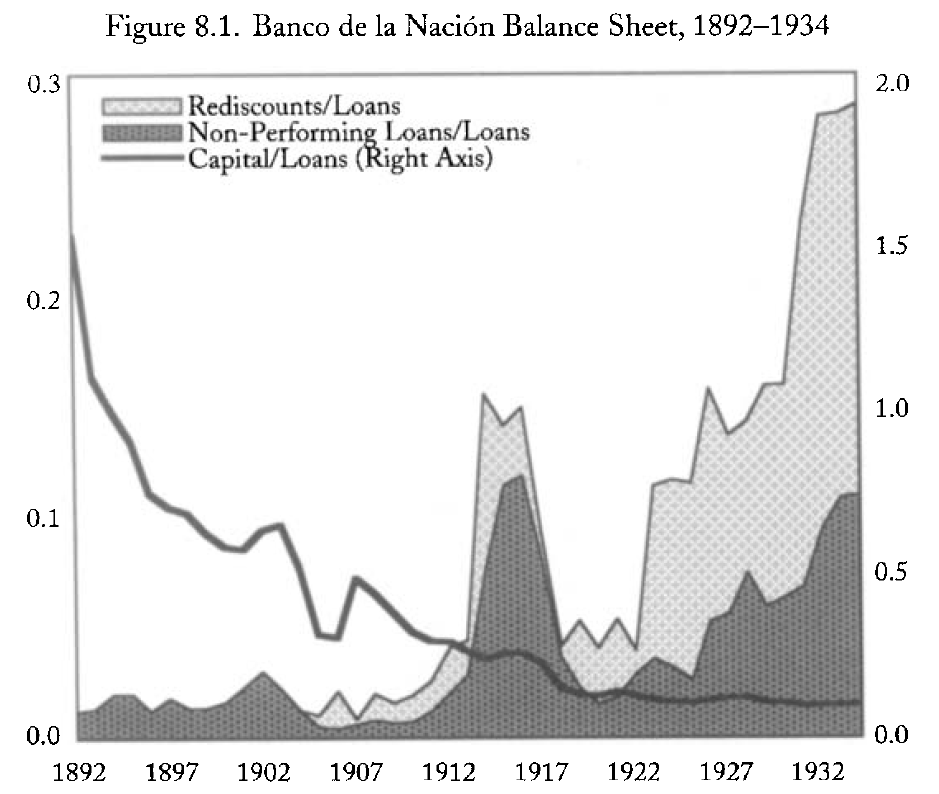
\includegraphics[scale=0.45]{uni2_post29}
   \label{fig:uni1_01}
\end{figure} 
  \end{frame}



  \begin{frame}\frametitle{El perfil del BNA (cont.)}
\begin{figure}[hxtbp]\vspace{0cm}
  \centering
  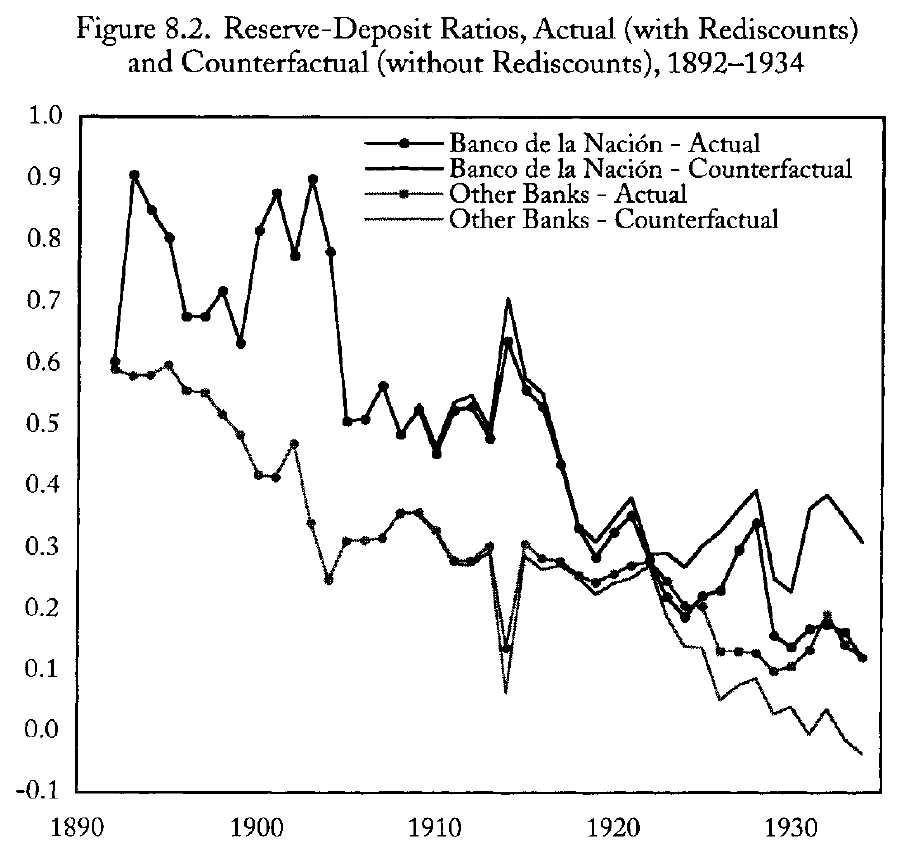
\includegraphics[scale=0.45]{uni2_post29_02}
   \label{fig:uni1_01}
\end{figure} 
  \end{frame}


  
 \begin{frame}\frametitle{Pequeños cambios, grandes consecuencias}
   \begin{block}{El deterioro de un sistema}
  El patrón oro era estable hasta 1914 combinado con prácticas
  conservadoras de \textit{inside-money}. En 1914, shocks externos y
  políticas domésticas alteraron las instituciones (prácticas). BNA y
  la CdC constituían \textbf{garantías implícitas} al sistema
  financiero pero como poderes de emergencia. Esto aumentó el
  potencial de riesgo moral sobre todo en torno a la actividad de
  prestamista de ultima instancia del BNA (no así de la CdC que se
  mantuvo conservadora) 
     \end{block}
      \end{frame}
  

 \begin{frame}\frametitle{Pequeños cambios, grandes consecuencias (cont.)}
   \begin{block}{El regreso al patrón oro}
 Antes de 1914 el patrón oro había funcionado sin fisuras logrando
 mantener el doble objetivo de la convertibilidad interna y externa
 bajo la tutela de una CdC creíble y banco Estatal acotado. Luego de
 1914, algunos elementos cruciales (de diseño/institucionales) de
 aquel sistema habían cambiado lo que impactó fuertemente sobre la
 salud del sistema bancario incluido el banco Estatal. Los agentes
 económicos percibían esto y la desconfianza no tardaría en manifestarse 
     \end{block}
      \end{frame}
  



\begin{frame}\frametitle{Pequeños cambios, grandes consecuencias (cont.)}
    \begin{itemize}\itemsep 10pt
      \item Cuando la CdC abrió sus puertas nuevamente en 1927 se
        produjeron una corrida interna masiva (depósitos), primero, a la que
        siguió una corrida externa masiva (oro)
        \item Las corridas obligaron a la CdC a abandonar la
          convertibilidad definitivamente --pérdidas de oro cerca de
          40\% menos de la tendencia.
          \item El BNA se había unido a los otros bancos en su
            calamitoso estado --reservas alrededor del 10\% de depósitos
                 \end{itemize}
      \end{frame}



\begin{frame}\frametitle{Nuevamente inconvertible: costos y beneficios}
    \begin{itemize}\itemsep 10pt
      \item Liberó la politica monetaria como modo de desacoplar
        precios locales de externos (deflacionario)
        \item El requisito de exportar oro aun seguía vigente (deuda
          externa) --decisión de política entre \textit{defaultear}
          deuda o imprimir papel sin respaldo
          \item Entre los costos, la disparada del tipo de cambio. Y
            aún restaba el pesado lastre de un sistema financiero en
            situación frágil
                 \end{itemize}
      \end{frame}

      



\begin{frame}\frametitle{Nuevamente inconvertible: costos y beneficios}
    \begin{itemize}\itemsep 10pt
      \item ¿Qué sucede si se elige un sistema de caja de conversión y
        ocurre un evento externo (crash, deflación)? Esto fue lo que
        Argentina descubriría  a la fuerza desde 1929
        \item Uno de los primeros impactos vino por el lado de precios
          de commodities y TIE --crisis de BP severa en 1929 y peso
          papel flotaba libre
          \item El producto creció en 1931 luego de varios años y en
            1934-35 había recuperado el nivel de 1929
            $\longrightarrow$ evidencia de rol de la PM (pero no de la PF)
                 \end{itemize}
      \end{frame}


\begin{frame}\frametitle{La Gran Depresión y Argentina}
    \begin{itemize}\itemsep 10pt
      \item Si bien la creación del BCRA en 1935 fue un hito muy
        importante, un cambio de régimen ya se había dado en 1931
        --CdC empezó a redescontar y así forjar un política monetaria
        propia e independiente
        \item Esta decisión tuvo importantes efectos en el hecho de
          que Argentina siguiera a otros países en un profundo abismo
          de deflación y recesión en 1931-33 (bajando las tasas de
          interés oportunamente)
                 \end{itemize}
      \end{frame}



      \begin{frame}\frametitle{La Gran Depresión y Argentina (cont.)}
        \begin{block}{El efecto Keynes}
          Una inyección directa de liquidez bajaría las tasas de
          interés y estimularía la demanda agregada y el producto
                   \end{block}
                   \begin{block}{El efecto Mundell}
                       Cambio decisivo en el régimen monetario posible
                       de convencer agentes de descartar expectativs
                       inflacionarias a través de un menor tasa de
                       interés real \textit{ex-ante}, mejora en la BP
                       y riesgo país
                     \end{block}                   
            
      \end{frame}




        \begin{frame}\frametitle{La Gran Depresión y Argentina (cont.)}
          \begin{itemize} \itemsep 15pt
          \item La realidad es que Argentina no utilizó la emisión de
            manera desmedida --presa tal vez de un temor
            inflacionario- y se limitó a destruir las expectativas
            deflacionarias a través de cambios institucionales
            \item La idea en Argentina a mediados de los 20's seguía
              siendo volver a la ortodoxia de la \textit{belle epoque}
              $\longrightarrow$ a pesar de haber sufrido la peor
              recesión de la historia (1914)
            \end{itemize}
      \end{frame}
      



        \begin{frame}\frametitle{La Gran Depresión y Argentina (cont.)}
          \begin{itemize} \itemsep 15pt
          \item Entre 1929 y 1932 el producto real en Argentina cayó
            un 14\% y la deflación fue del 6\% --más del 30\% de caida
            en producto real y 20\% de deflación para EEUU y
            Canadá. También comparada favorablamente con resto de Latam
            \item Un tema relevante es que Argentina pudo optar por
              este cambio de política monetaria $\longrightarrow$ 80\%
              de la BM respaldada por oro
                 \item El mix de política incluía ``finanzas solidas'' en
                lo fiscal y sistema monetario fiduciario no ortodoxo
                         \end{itemize}
      \end{frame}
      



  \begin{frame}\frametitle{La Gran Depresión y Argentina (cont.)}
          \begin{itemize} \itemsep 15pt
          \item En la \textbf{política fiscal} no hubo cambios
            principales $\longrightarrow$ postura fiscal ortodoxa
            (presupuesto equilibrado)
            \item Durante los 30s, los principales impuestos seguían
           vinculados con el comercio exterior --debido a la
           ciclicidad de los ingresos y la rigidez de gastos, hubo
           varios deficits
           \item No hubo política de déficit expansivos --sino de
             mayores impuestos para lograr balance/superavits
           
                         \end{itemize}
      \end{frame}








      
  \begin{frame}\frametitle{La Gran Depresión y Argentina (cont.)}
\begin{figure}[hxtbp]\vspace{0cm}
  \centering
  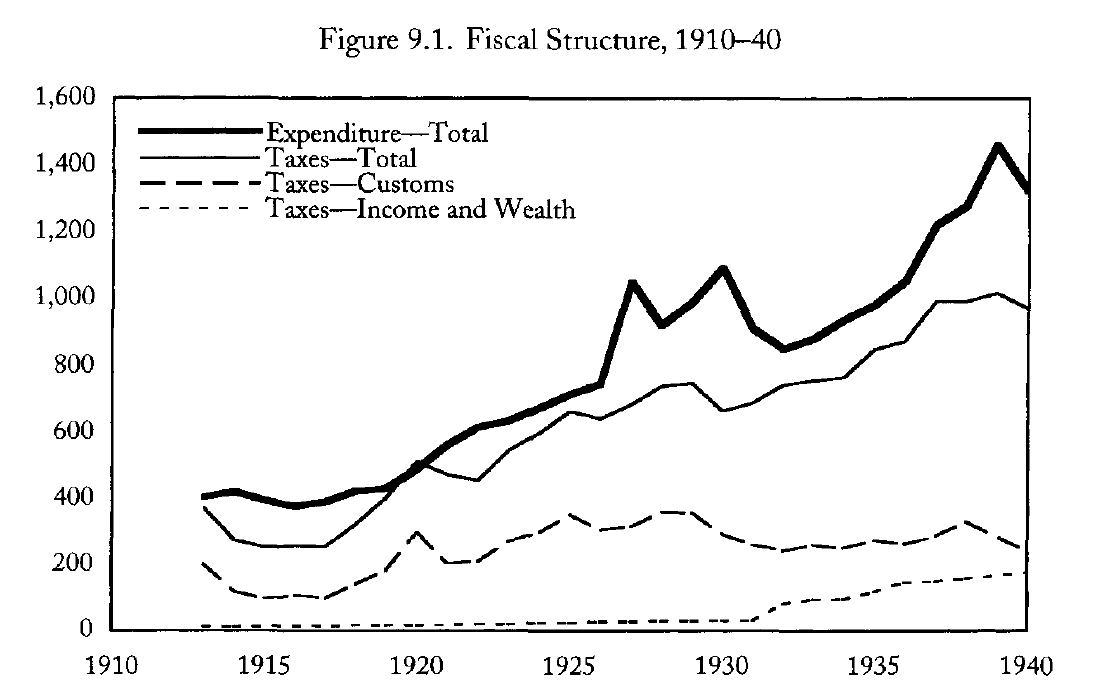
\includegraphics[scale=0.45]{uni2_post29_03}
   \label{fig:uni1_01}
\end{figure} 
  \end{frame}




\begin{frame}\frametitle{La Gran Depresión y Argentina (cont.)}
          \begin{itemize} \itemsep 15pt
          \item Muchos países de América latina defaultearon sus
            deudas (aumentadas por deflación y depreciación) pero no
            fue el caso de Argentina
            \item La unica salida que le quedaba la gobierno --no
              tenía acceso al mercado de K ni tampoco podía aumentar
              impuestos en corto plazo $\longrightarrow$ echar mano de
              reservas de oro en CdC.
              \item Seguir esta ortodoxia fiscal sería costosa en el
                mediano/largo plazo (baja de BM, deflación)
                         \end{itemize}
      \end{frame}
  



\begin{frame}\frametitle{La Gran Depresión y Argentina (cont.)}
          \begin{itemize} \itemsep 15pt
          \item Una característica central de la política monetaria Argentina durante el
            período inter-guerras es que se mantuvo una ortodoxia
            monetaria bastante importante --incluso durante la
            suspensión de la convertibilidad
            \item Esto es aún más destacable siendo que muchos países
              pasaron por inflaciones e hiperinflaciones --no hubo un
              plan sistemático de emisión descontrolada para financiar
              déficit
              \item Notar que aún sin conversión se siguió la regla
                --flotación de TC
                         \end{itemize}
      \end{frame}
  

      

  \begin{frame}\frametitle{La Gran Depresión y Argentina (cont.)}
\begin{figure}[hxtbp]\vspace{0cm}
  \centering
  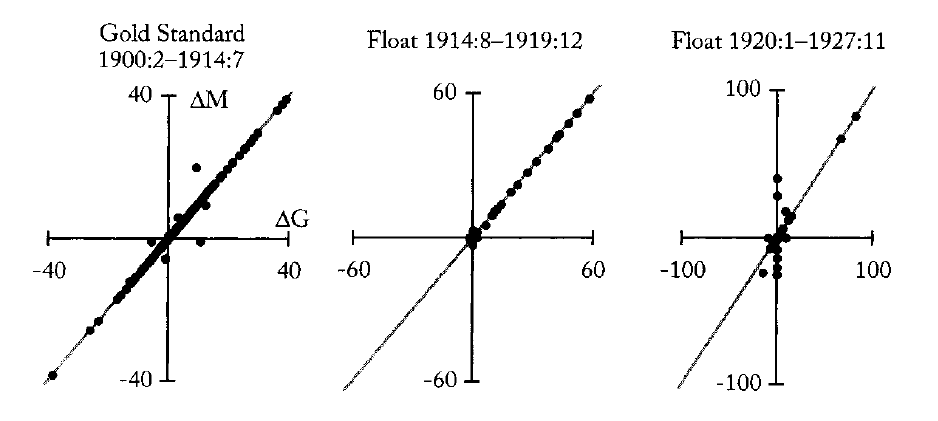
\includegraphics[scale=0.8]{uni2_post29_04}
   \label{fig:uni1_01}
\end{figure} 
  \end{frame}


        

  \begin{frame}\frametitle{La Gran Depresión y Argentina (cont.)}
\begin{figure}[hxtbp]\vspace{0cm}
  \centering
  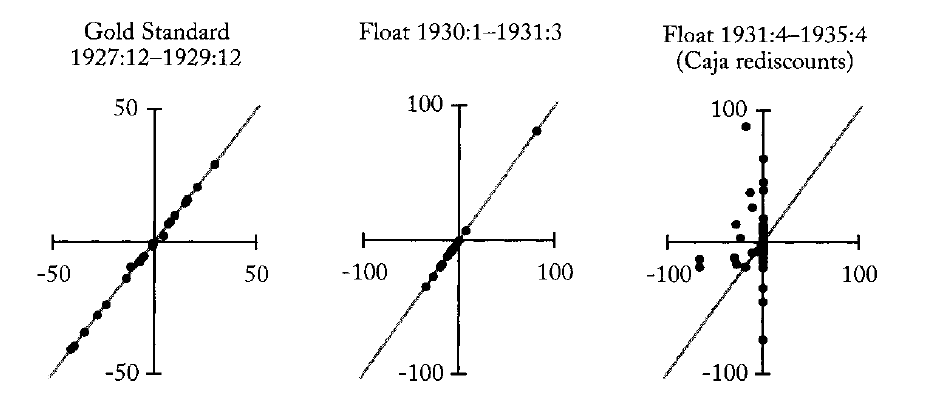
\includegraphics[scale=0.8]{uni2_post29_05}
   \label{fig:uni1_01}
\end{figure} 
  \end{frame}


\begin{frame}\frametitle{La Gran Depresión y Argentina (cont.)}
          \begin{itemize} \itemsep 15pt
          \item La estrategia del patrón oro de mano única --tan
            curiosa y original adoptada- era consistente con el
            objetivo de largo plazo de retomar convertibilidad  a la
            par $\longrightarrow$ entre 1914 y mitad de los 20s
            Argentina había usado el enorme stock de oro de manera
            cuidadosa
            \item ¿El costo de esto? El tipo de cambio no se depreció
              de manera masiva hasta 1929 $\longrightarrow$ pero si
              luego de esa Gran Depresión
                         \end{itemize}
      \end{frame}
  
  

    

  \begin{frame}\frametitle{La Gran Depresión y Argentina (cont.)}
\begin{figure}[hxtbp]\vspace{0cm}
  \centering
  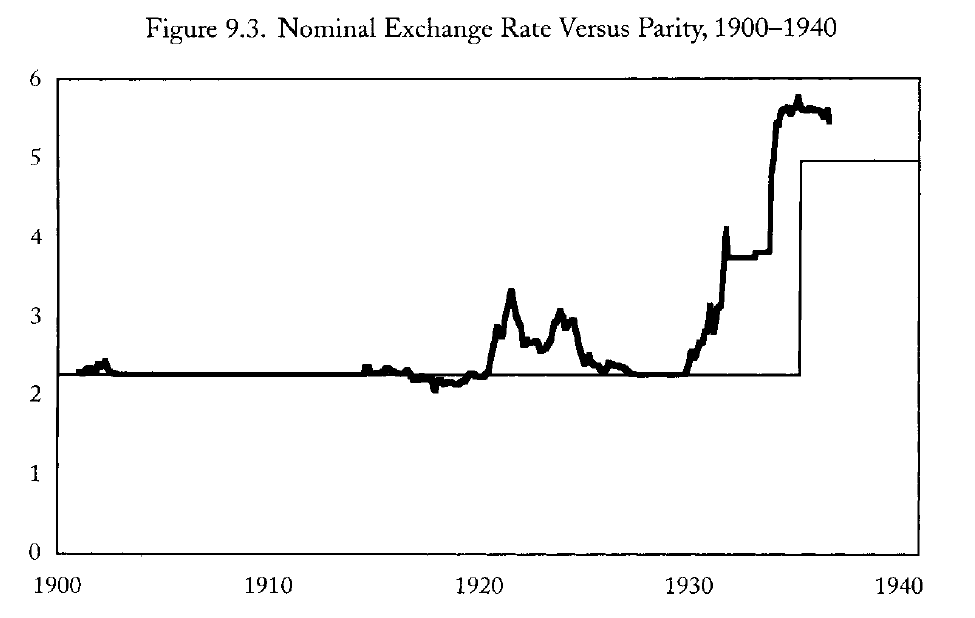
\includegraphics[scale=0.6]{uni2_post29_06}
   \label{fig:uni1_01}
\end{figure} 
  \end{frame}




\begin{frame}\frametitle{La Gran Depresión y Argentina (cont.)}
          \begin{itemize} \itemsep 15pt
          \item ¿Qué cambió alrededor de los años de la Gran
            Depresión? En primer lugar, y mas importante, fue que
            \textbf{a pesar de no haber cambios en reservas de oro, la
              CdC frecuentemente cambiaba la BM a través de
              redescuentos}.
            \item Así fue como la base del régimen monetario pasaría
              de metálico a fiduciario en el año 1931
              $\longrightarrow$ a fin de año moneda fiduciaria pasó de
              0\% a 30\% de la BM --la cara espejada fue que el
              respaldo en oro de la BM cayó de 78\% a 43\%.
                         \end{itemize}
      \end{frame}


\begin{frame}\frametitle{La Gran Depresión y Argentina (cont.)}
          \begin{itemize} \itemsep 15pt
          \item Hay un movimiento casi paralelo entre que la CdC
            empezó a redescontar --motivaciones
            fiscales- y el aumento del tipo de cambio (pasó de 28\% a
            80\% de la paridad
            \item Las expectativas de los agentes incorporaron estos
              cambios --desacople de oro y moneda- como permanentes
              $\longrightarrow$ en 1931-35 el cambio promedio anual en
              oro fue de -6.7 millones (en pesos papel) mientras que la BM aumentó en
              0.6 millones (en pesos papel)
              \item Esta PM heterodoxa y precoz significó un enorme
                cambio respecto de la ortodoxia monetaria pero evitó
                una crisis económica gigantesca
                         \end{itemize}
      \end{frame}
  

\begin{frame}\frametitle{La Gran Depresión y Argentina (cont.)}
          \begin{itemize} \itemsep 15pt
          \item Hay un movimiento casi paralelo entre que la CdC
            empezó a redescontar --esencialmente por motivaciones
            fiscales- y el aumento del tipo de cambio (pasó de 28\% a
            80\% de la paridad
            \item Las expectativas de los agentes incorporaron estos
              cambios --desacople de oro y moneda- como permanentes
              $\longrightarrow$ en 1931-35 el cambio promedio anual en
              oro fue de -6.7 millones (en pesos papel) mientras que la BM aumentó en
              0.6 millones (en pesos papel)
              
                         \end{itemize}
      \end{frame}
  
      

\begin{frame}\frametitle{La Gran Depresión y Argentina (cont.)}
          \begin{itemize} \itemsep 15pt
          \item La commbinación de dos medidas adoptadas en los
            primeros años 30 fijaron un marco de acción diferente para
            toda la PM argentina a futuro:
            \begin{itemize}\itemsep10pt \medskip
            \item Autorización de redescuentos de la CdC al sistema
              bancario
              \item Autorizar la emisión del ``Empréstito Patriótico''
                al Gobierno --autorizar emitir billetes contra títulos
                del Estado
              \end{itemize}
              \item Esto sumado al control de cambios impuesto en 1931
                que se reforzó en 1933 con permisos de importación y
                tipos de cambios múltiples
                                       \end{itemize}
      \end{frame}
  


      \begin{frame}\frametitle{La Gran Depresión y Argentina (cont.)}
          \begin{itemize} \itemsep 15pt
          \item El control de cambios permitió controlar parcialmente
            la evolución del tipo de cambio --pero con el continuo
            drenaje de reservas el tipo de cambio siguió subiendo
            \item El sector bancario sufrió lenta y
              gradual drenaje de depósitos. Hacia 1933-34 casi todos
              los bancos tenían corridas
              \item El Estado -fiscal- muy afectado por restricción de
              comercio que requirió de reforma tributaria.
              \item El BNA ahora debería resguardar a los dos
                principales sistemas económicos --bancario, Estado. El
                sistema quedó al borde del colapso .
                                       \end{itemize}
      \end{frame}
  
      
      

      
      
      
\end{document}

      